% Learned-only relay-drone delivery: set-based CTDE SAC against a geometric relay rule (English)
% Target version: v5.10 (26_10_01_00). Supersedes paper_en_v3_26_08_31_19.tex.
% Compile: pdflatex (run twice for references to figures)
\documentclass[12pt]{article}
\usepackage[margin=1in]{geometry}
\usepackage{setspace}
\usepackage{amsmath, amssymb}
\usepackage{booktabs}
\usepackage{graphicx}
\usepackage{url}
\doublespacing
\pagestyle{empty}



\title{Learned-Only Multi-Agent Control of a Relay-Drone Network for\\
Disaster Relief Delivery: What a Set-Based Policy Wins and Where a\\
Geometric Rule Still Leads}
\author{Kwangjong Ko \and Hyunseok Choi \and Taesu Cheong\thanks{Corresponding author.}\\
Department of Industrial and Management Engineering, Korea University}
\date{}

\begin{document}
\maketitle

\begin{abstract}
In a disaster zone without communication infrastructure, a fleet of homogeneous drones must
deliver relief supplies while every aircraft stays connected to the control centre through a
multi-hop relay chain formed by the fleet itself. A drone that holds a relay position cannot
deliver, so the fleet trades throughput for reach at every decision. We study the learned-only
setting: a single set-based policy, trained once with three to four drones on twenty to eighty
destinations, is deployed without retraining on fleet sizes, destination counts and depot
positions it has never seen. Connectivity is a hard constraint enforced by a minimal-perturbation
projection; a high-level manager assigns each drone a destination, a return or a relay slot every
twenty steps, deciding drones autoregressively from the farthest inward; the low-level controller
is straight-line flight. The manager is trained with discrete soft actor-critic whose entropy
target is annealed from $0.6\log n$ to $0.25\log n$, regularised toward a geometric relay rule,
and selected on a held-out makespan score.

Against the strongest learning-free baseline we could build, a geometric relay rule augmented
with a deadlock-escape mechanism, the learned policy is evaluated by pairing the two methods on
identical instances and testing the paired differences with the Wilcoxon signed-rank test on
200 to 240 rollouts per configuration. The learned policy completes every instance in all three
configurations where the rule fails 3 of 240 and 10 of 200. On the unseen five-drone
configuration it is faster by 54 steps in paired median ($p < 10^{-4}$); on the training
configuration the two are tied ($+18$, $p = 0.17$); on the unseen three-drone configuration the
rule is faster by 40 steps ($p < 10^{-4}$). A high-level decision costs 3.5\,ms at four drones,
against 600--1200\,s for a time-expanded MILP that finds no feasible plan beyond six destinations.
We trace the three-drone deficit to relay assignment: the policy stations 0.78 relays where the
rule stations 1.39, and overriding only the rule's choice of \emph{which} drone relays recovers
the entire gap. Five training-side interventions aimed at that decision, spanning imitation
weighting, reward credit for relays, checkpoint selection and per-drone critics, all failed, and
we report them.
\end{abstract}

\section{Introduction}

Relief delivery after a disaster is a routing problem with an unusual coupling. Communication
infrastructure is gone, so each drone can talk to the control centre only within a direct range
$R$, or through other drones that forward its traffic. Every aircraft must remain connected at
all times, for live video during unloading and for tracking; a drone that stations itself as a
relay extends the fleet's reach at the cost of its own deliveries. The fleet therefore makes,
continuously, a joint decision about who delivers and who relays, and the makespan of serving
all demand depends on that decision as much as on the routes.

Exact optimisation does not scale here. A time-expanded mixed-integer model that enforces
$n$-hop connectivity in every period has, for three drones and ten destinations on a 98-metre
lattice, about $11{,}000$ binaries and finds no feasible plan in ninety minutes
(Section~\ref{sec:milp}). A geometric rule that places relays at fixed fractions of the line
from the depot to the lead drone is fast and, once a deadlock-escape mechanism is added,
completes almost every instance. It is the baseline any learned method must beat, and this paper
reports carefully where a learned policy does and does not.

Our contribution is a learned-only controller and an honest account of it. The controller is
a set-based, drone-count-agnostic manager trained once and deployed on unseen fleet sizes and
depot positions. Its wins are unambiguous on completion rate, on the unseen five-drone
configuration, and on inference cost. Its loss on the three-drone configuration is measured,
diagnosed to a single decision, and shown to resist five plausible fixes. We also document two
methodological corrections that changed our conclusions: that comparing makespan only over the
episodes each method completed favours the method that gives up on hard instances, and that
forty-rollout samples cannot support claims about tails or about differences of thirty steps.

\section{Related Work}

Routing with drones has been studied since the flying-sidekick problem of Murray and Chu (2015)
and its multi-drone extensions (Murray \& Raj 2020; Agatz et al.\ 2018; Dorling et al.\ 2017);
none of these models communication. UAV relay positioning is its own literature (Zeng, Zhang \&
Lim 2016; Yanmaz 2022; Ding et al.\ 2022), but there the relays are the mission, not a role the
delivery fleet takes on and gives up. Multi-UAV exploration under communication limits (Cesare
et al.\ 2015) is the closest in spirit. On the learning side we build on soft actor-critic
(Haarnoja et al.\ 2018), centralised critics for decentralised execution (Lowe et al.\ 2017;
Foerster et al.\ 2018), value decomposition (Sunehag et al.\ 2018; Rashid et al.\ 2018), options
as a semi-Markov decision process (Sutton, Precup \& Singh 1999), invalid-action masking (Huang
\& Onta\~{n}\'{o}n 2022) and safe-action projection (Dalal et al.\ 2018). Learned solvers for
min-max multi-vehicle routing (Park, Kwon \& Park 2023) show set-based policies generalising
across problem sizes, which is the property we need across fleet sizes.

\section{Problem Statement}

A control centre sits at $c \in [0,1000]^2$ and $M$ destinations $d_1,\dots,d_M$ lie within
$0.9\,N R$ of it, where $N$ is the number of drones and $R = 300$\,m the communication range.
Each drone flies at $v = 13.89$\,m/s, carries $Q = 5$ units, unloads one unit per destination in
$S = 10$ steps, and reloads to $Q$ at the centre in $S$ steps; the interaction radius is 25\,m
and one step is one second. The fleet must stay connected: at every step the graph with the
centre and the drones as vertices and edges between vertices within $R$ must be connected. The
objective is the makespan, the step at which the last destination is served. We call the
$N = 4$, $M = 50$, fixed-depot setting the \emph{standard} configuration; the policy is trained
with $N \in \{3,4\}$, $M \in [20,80]$ and a random depot, and evaluated in addition on two
configurations it never saw, $N = 3$, $M = 30$ and $N = 5$, $M = 50$, both with random depots.

\section{Method}

\subsection{Connectivity as a hard constraint}

A reward penalty for disconnection punishes situations no action can prevent: a drone that is
stationary while unloading is stranded when a teammate departs. Connectivity is therefore
enforced by projection. Each commanded displacement is scaled by the largest factor in $[0,1]$
that keeps the fleet connected, with ties between drones broken at random. The scaled-away
distance is recorded as a \emph{blocked} drone-step; blocked steps turn out to be the diagnostic
signature of under-relaying (Section~\ref{sec:diag}). No connectivity loss occurred in any
training episode or evaluation rollout reported here.

\subsection{Hierarchy and the manager's action space}

A manager acts every $20$ steps, or as soon as a drone's goal becomes invalid, and assigns each
drone one of $K = 7$ discrete options: one of five candidate destinations (the three nearest
unserved ones and the two farthest from the centre), a return to the centre, or a relay slot.
Relay slots lie on the segment from the centre to the lead drone at multiples of $0.9R$; the
environment assigns the slot, so the policy's relay decision is only \emph{whether} a drone
relays. The low-level controller is straight-line flight to the goal; a learned worker was tried
in earlier versions and was harmful. Between manager decisions the environment is a semi-Markov
decision process and the manager's transitions store the discounted option return.

\subsection{Set-based, drone-count-agnostic manager}

The manager encodes each drone as a set of entities: its own state (10 features), its five
candidates (6 features each), its peers (9 features each, of which four are a one-hot of the
peer's current role), and its relay slot (4 features). Attention pooling over candidates and
over peers produces a per-drone embedding from which a pointer head scores the candidates and a
fixed head scores return and relay. Nothing in the network depends on $N$ or $M$, which is what
allows a single set of weights to run on fleet sizes it never saw. Invalid options are masked.

Decisions are \emph{autoregressive}: drones are ordered by distance from the centre, farthest
first, and after each drone's option is sampled its new role is written into the peer features
seen by the drones decided after it. A formation of one lead and $k$ relays arises only by
coincidence under independent per-drone sampling but can be matched deliberately under
sequential decisions. The price is $N$ sequential network calls per decision.

\subsection{Training}

The manager is trained with discrete soft actor-critic. A twin-Q critic with attention across
drone embeddings outputs per-drone action values whose mean over drones is regressed on the
team return; the actor loss is the standard expectation form. Three ingredients matter.

\emph{Entropy target.} The conventional target of $0.6 \log n_{\mathrm{valid}}$ holds the
temperature at 2--3 and keeps the policy too random to hold a multi-step formation, while that
same randomness is the only mechanism by which a deadlocked fleet escapes. Annealing the target
linearly from $0.6 \log n$ to $0.25 \log n$ over the first 400 episodes lowered the standard-
configuration makespan from 1{,}418 to the 900s; it is the single largest contributor.

\emph{Rule regularisation.} A cross-entropy term with weight 2.0 pulls the policy toward the
action the geometric rule would take, wherever that action is unmasked. Removing it collapses
completion early in training and costs 300--400 steps of makespan.

\emph{Configuration randomisation.} Training samples $N$, $M$ and the depot position afresh
every episode. Removing it makes the standard configuration 44 steps faster and the unseen
three-drone configuration 646 steps slower.

Checkpoints are scored every 50 episodes on 80 held-out instances with a 3{,}000-step budget by
$100\,f + 40\,(1 - \bar{t}/3000)$, where $f$ is the completion rate and $\bar{t}$ the mean steps,
so that one percentage point of completion equals 75 steps; the earlier weight of 10 made it
equal 300 and discarded fast checkpoints for a single missed instance. Training stops after
eight consecutive evaluations without improvement or at 1{,}000 episodes.

\section{Baselines and Evaluation Protocol}

\subsection{Five learning-free baselines}

We compare against a greedy assignment with no relays, a geometric relay rule, the same rule with
a deadlock-escape mechanism, and two fixed-relay policies that permanently dedicate one or two
drones. The geometric rule stations relays along the depot-to-lead segment and is deterministic;
it deadlocks on 38\% of standard instances. The escape mechanism swaps the lead drone whenever the
fleet has been stalled for 60 steps and holds the new assignment for 40 steps, which lifts
completion to 97--100\%. Table~\ref{tab:base} reports all five on all three configurations; the
augmented rule is the only credible baseline and every comparison below is against it.

\begin{table}[h]
\centering
\caption{Learning-free baselines: completion rate and mean makespan over completed episodes.
Standard configuration 120 rollouts, unseen configurations 40.}
\label{tab:base}
\begin{tabular}{lccc}
\toprule
Method & 4 drones / 50 dest. & 3 / 30 (unseen) & 5 / 50 (unseen) \\
\midrule
Greedy, no relay & 0\% & 0\% & 25\% $\cdot$ 516 \\
One fixed relay & 0\% & 2.5\% & 40\% $\cdot$ 544 \\
Two fixed relays & 3.3\% $\cdot$ 914 & 52.5\% $\cdot$ 875 & 65\% $\cdot$ 611 \\
Geometric relay rule & 61.7\% $\cdot$ 810 & 95\% $\cdot$ 581 & 92.5\% $\cdot$ 598 \\
Rule + deadlock escape & 98.3\% $\cdot$ 887 & 100\% $\cdot$ 607 & 92.5\% $\cdot$ 623 \\
Learned policy (ours) & 100\% $\cdot$ 911 & 100\% $\cdot$ 689 & 100\% $\cdot$ 593 \\
\bottomrule
\end{tabular}
\end{table}

\subsection{Paired comparison}

Averaging makespan over the episodes each method completed is biased: the hard instances a
method gives up on drop out of its average and stay in the other's. A second problem is that
the learned policy has a heavy tail; one 8{,}336-step rollout moves a 40-instance mean by 110
steps, and the same weights measured three times on the standard configuration gave means of
899, 985 and 950. We therefore roll both methods out on the same instances with the same
repetition index, keep the pairs both completed, and report the median paired difference, the
win--loss count and the Wilcoxon signed-rank $p$-value, with 240 rollouts on the standard
configuration and 200 on each unseen one. Inference samples from the policy; the greedy argmax
has the same median and a far heavier tail (maximum 8{,}482 against 2{,}538 on 120 rollouts),
which confirms that sampling is the deadlock-escape mechanism. All rollouts have a 10{,}000-step
budget and no early termination.

\section{Results}

\subsection{Three configurations}

\begin{table}[h]
\centering
\caption{Learned policy against the rule with escape on identical instances. Positive paired
difference means the learned policy is slower. $p$ from the Wilcoxon signed-rank test.}
\label{tab:main}
\resizebox{\textwidth}{!}{%
\begin{tabular}{lcccccc}
\toprule
Configuration & Rollouts & Completed rule / ours & Median rule / ours & Paired diff. & Wins--losses & $p$ \\
\midrule
4 / 50, seen & 240 & 237 / \textbf{240} & 866 / 879 & $+18$ & 109--127 & 0.17 \\
3 / 30, unseen & 200 & 200 / 200 & \textbf{572} / 617 & $+40$ & 73--127 & $<10^{-4}$ \\
5 / 50, unseen & 200 & 190 / \textbf{200} & 570 / \textbf{532} & $\mathbf{-54}$ & 141--45 & $<10^{-4}$ \\
\bottomrule
\end{tabular}}
\end{table}

The learned policy completes every instance in every configuration; the rule leaves 3 of 240
and 10 of 200 unfinished within the budget. On the unseen five-drone configuration the learned
policy is 54 steps faster in paired median and wins 141 pairs of 186. On the training
configuration the two are indistinguishable: two independent 120-rollout measurements gave
paired medians of $+24$ and $+17$, neither significant, and the pooled $p$ is 0.17. On the
unseen three-drone configuration the rule is 40 steps faster and the difference is significant.
Figure~\ref{fig:paired} shows the full distributions.

\begin{figure}[h]
\centering
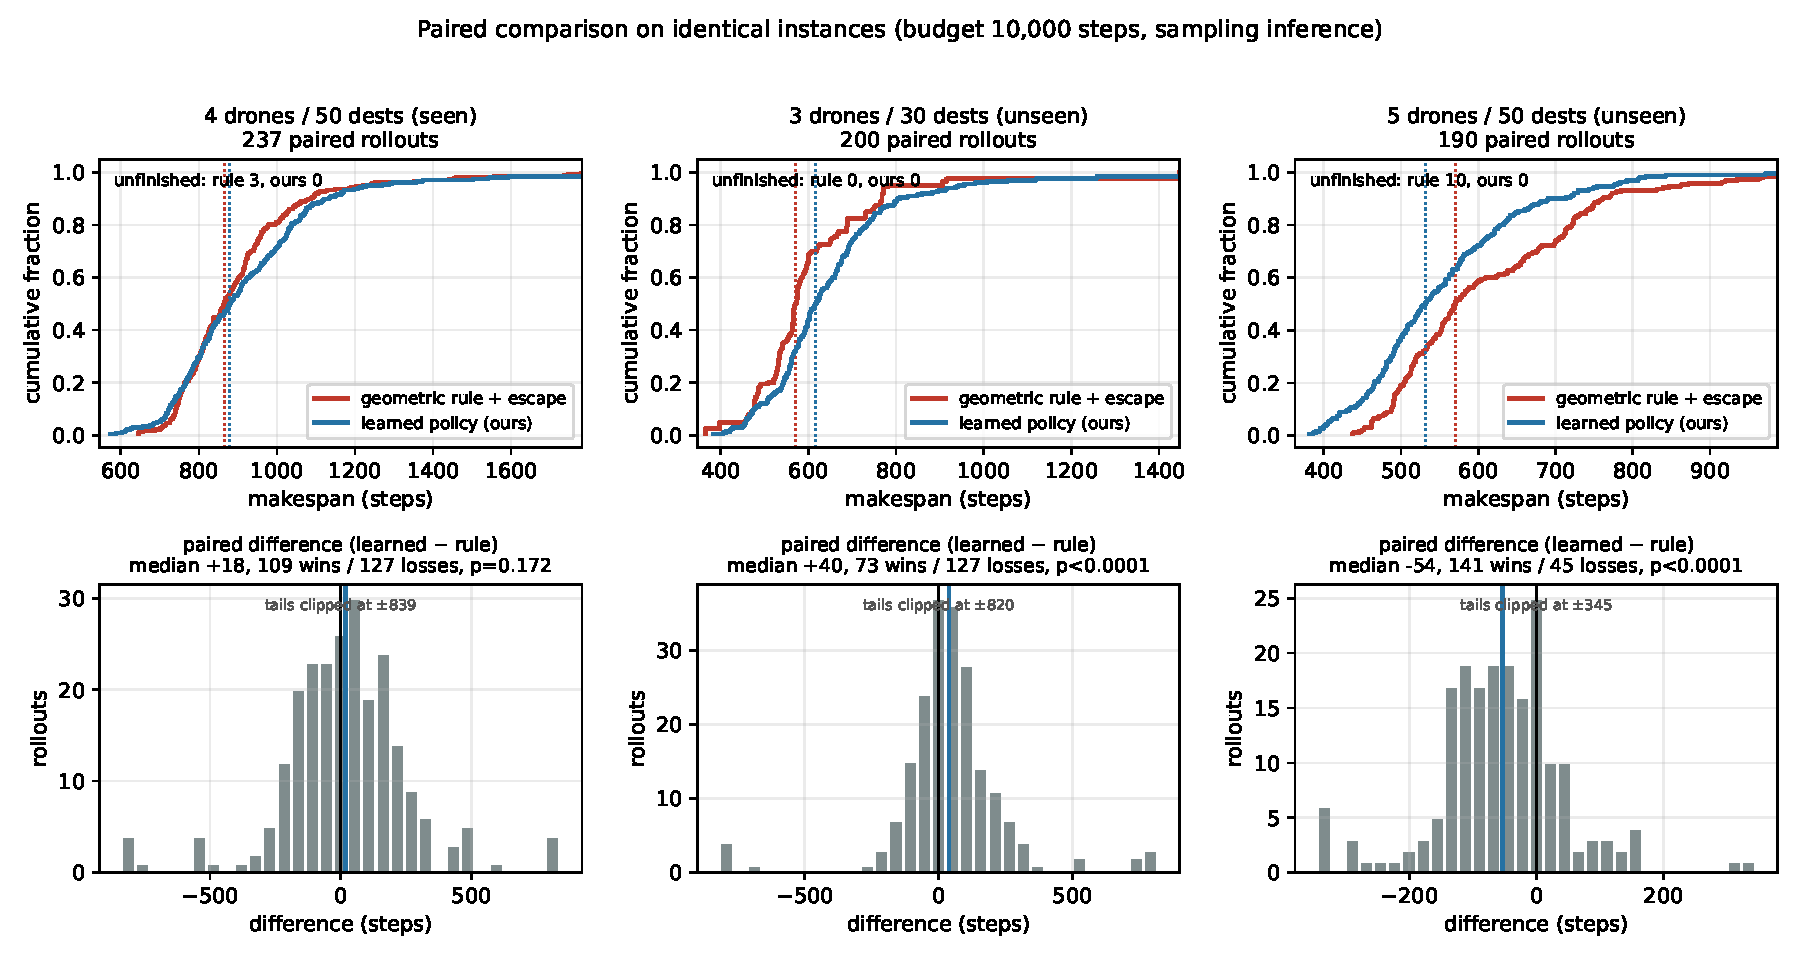
\includegraphics[width=\textwidth]{../../figures/paired_compare_v5_26_09_27_13.pdf}
\caption{Cumulative makespan distributions (top, dotted lines at medians) and paired
differences (bottom) for the three configurations.}
\label{fig:paired}
\end{figure}

\subsection{Tails}

The direction of the tail follows the direction of the median. Where drones are scarce the
learned policy's worst case is worse than the rule's; where they are plentiful it is better.

\begin{table}[h]
\centering
\caption{Standard deviation and maximum of completed makespan.}
\label{tab:tail}
\begin{tabular}{lcc}
\toprule
Configuration (rollouts) & Rule sd / max & Ours sd / max \\
\midrule
4 / 50 (240) & 188 / 2{,}014 & 521 / 8{,}336 \\
3 / 30 (200) & 172 / 1{,}447 & 382 / 5{,}395 \\
5 / 50 (200) & 150 / 1{,}734 & 111 / 1{,}101 \\
\bottomrule
\end{tabular}
\end{table}

The 8{,}336-step event is rare: one in 960 standard rollouts exceeded 2{,}500 steps, and the same
instance run twice gave 702 and 8{,}336, so it is a stochastic stall, not an instance property.
An inference-side intervention that resamples the policy at temperature 5 whenever the fleet has
been stalled for 120 steps cuts the 600-rollout maximum from 2{,}361 to 1{,}541 and the share of
rollouts above 1{,}500 steps from 1.2\% to 0.3\% at no median cost (paired $-7$, $p = 0.43$); the
tail reduction itself is not yet significant (Fisher $p = 0.18$).

\subsection{Inference cost}

A high-level decision costs 0.08\,ms for the rule, 1.52\,ms for the learned policy without
autoregression and 3.52\,ms with it, at four drones on a CPU; the autoregressive cost grows at
0.93\,ms per additional drone. A 900-step episode spends 0.158\,s in the manager. The
time-expanded MILP of Section~\ref{sec:milp} needs 600--1{,}200\,s on instances with four to six
destinations.

\subsection{Ablations}

Each component was removed in turn with two seeds. Because the same configuration trained four
times spans 919--979 steps on the standard configuration, only differences above 70--80 steps
between two-seed means are meaningful; those are in bold.

\begin{table}[h]
\centering
\caption{Ablation: completion and mean makespan, two seeds, difference from the full method in
parentheses.}
\label{tab:abl}
\resizebox{\textwidth}{!}{%
\begin{tabular}{lccc}
\toprule
Removed & 4 / 50 & 3 / 30 & 5 / 50 \\
\midrule
Nothing (full method) & 120/120 $\cdot$ 927 & 40/40 $\cdot$ 755 & 40/40 $\cdot$ 574 \\
Residual penalty & 120/120 $\cdot$ 899 ($-28$) & 40/40 $\cdot$ 718 ($-37$) & 40/40 $\cdot$ 582 ($+8$) \\
Autoregression & 120/120 $\cdot$ 1{,}022 ($\mathbf{+94}$) & 40/40 $\cdot$ 710 ($-46$) & 40/40 $\cdot$ 607 ($+33$) \\
Entropy annealing & 120/120 $\cdot$ 1{,}056 ($\mathbf{+128}$) & 40/40 $\cdot$ 774 ($+19$) & 40/40 $\cdot$ 635 ($+61$) \\
Config. randomisation & 120/120 $\cdot$ 883 ($-44$) & 40/40 $\cdot$ 1{,}402 ($\mathbf{+646}$) & 40/40 $\cdot$ 642 ($+68$) \\
Rule regularisation & 118/120 $\cdot$ 1{,}246 ($\mathbf{+320}$) & 39/40 $\cdot$ 1{,}163 ($\mathbf{+408}$) & 40/40 $\cdot$ 666 ($\mathbf{+92}$) \\
\bottomrule
\end{tabular}}
\end{table}

Rule regularisation is essential; configuration randomisation is what generalisation costs on
the training configuration and buys on the unseen one; entropy annealing and autoregression
matter on the standard configuration. The residual penalty is neutral, and a first reading that
called it harmful was retracted once four runs of the same configuration were available.

\section{Why the Three-Drone Configuration Is Slower}
\label{sec:diag}

With three drones and destinations up to 810\,m away, a far delivery needs two relays, leaving
one deliverer. On 40 three-drone instances the rule stations 1.39 relays on average and the
learned policy 0.78; the policy sends 1.78 drones to deliver against the rule's 1.32, and the
connectivity projection blocks 1{,}289 drone-steps against 160. The policy under-relays and is
dragged.

A probe isolates the cause. Overriding only the policy's relay assignments with the rule's,
while leaving its destination choices intact, cuts blocked steps by 60\% and recovers the whole
gap (paired median $-44$ against the unmodified policy, versus $-43$ for the rule itself).
Matching only the rule's relay \emph{count}, with the drones chosen by the policy's own relay
probabilities, collapses the tail (maximum 4{,}904 to 1{,}083) but recovers only 14 steps of
median. The tail is a matter of how many drones relay; the median is a matter of which.

The information needed for that choice is present: a two-layer classifier predicts the rule's
per-drone relay decision from the policy's 41 observation features with 85\% accuracy against a
51\% majority baseline. What is missing is the training signal. The critic's greedy policy, the
per-drone argmax of its action values, loses to the actor 0--40 with a median makespan of 2{,}022
against 670, even when actor and critic are taken from the same episode: the critic is trained
only through the mean of per-drone values against the team return, so the decomposition is
under-determined and the actor's competence comes from the entropy-regularised policy gradient
and the rule term, not from an accurate per-drone value.

\subsection{Five interventions that did not close the gap}

We report these because each was the natural next step given the diagnosis and each failed.
Values are paired medians against the rule on the three-drone configuration, 200 rollouts; the
full method sits at $+40$.

\begin{table}[h]
\centering
\caption{Training-side interventions aimed at relay assignment. Two seeds each.}
\label{tab:fail}
\resizebox{\textwidth}{!}{%
\begin{tabular}{llc}
\toprule
Intervention & Mechanism & 3 / 30 paired median \\
\midrule
Drop autoregression and residual penalty & simpler policy, $2.3\times$ faster & $+62$, $+132$ \\
Rule-regularisation weight $\times 3$ on relay actions & stronger imitation of relaying & $+54$, $+56$ \\
Uniform rule-regularisation weight $4.0$ & stronger imitation overall & $+23$, $+39$ \\
Per-drone reward credit to path relays & credit assignment & $+36$, $+58$ \\
Mixed holdout (half three-drone) for selection & selection sees the target & $+37$, $+68$ \\
Zero-sum credit taken from the deliverer & credit without an incentive to relay & $+91$, $+126$ \\
\bottomrule
\end{tabular}}
\end{table}

Imitation weighting raised the relay share during training from 0.24 to 0.30 but not toward
the rule's 0.44. Reward credit raised it to 0.36 and reversed the five-drone advantage from
$-54$ to $+60$: a drone parked on a busy path collects credit for every delivery that passes,
so relaying became an end in itself; the zero-sum variant removed that incentive and instead
starved delivery learning. A control arm that changed only the critic's target to per-drone
rewards, without any credit, was unstable across seeds and lost the five-drone advantage on its
own. Selecting checkpoints on a mixed holdout improved the standard configuration (arm mean from
$+19$ to $0$, one weight reaching $-37$) but not the three-drone one, and a sweep over every saved
checkpoint of four runs found none closer than 40 steps to the rule on a fresh seed range. The
deficit is a property of the policy, not of selection, reward magnitude or observation.

\section{A Time-Expanded MILP as a Reference}
\label{sec:milp}

For small instances we solve a time-expanded network on a 98.2-metre lattice with periods of 10
steps, single-commodity flow for connectivity in every period and a symmetry-breaking cut; the
formulation and its proofs are in a companion document. With three drones the model returns a
plan for four and six destinations, which replayed in the simulator beats the rule by 7 and 9
steps, and returns nothing for ten destinations in ninety minutes. Its optimum is a restriction
of the continuous problem and not a bound on it. A certified lower bound through a cell
relaxation was attempted and abandoned: on the four-destination instance the relaxation's dual
bound after seven minutes is 40 steps, below the trivial analytic bound of 60, because testing
communication by the minimum distance between cells inflates a three-hop chain's reach from
900\,m to 1{,}317\,m; keeping that inflation below 10\% needs 21-metre cells and roughly
$7 \times 10^{7}$ flow variables. The difficulty of the problem lies entirely in the connectivity
constraint, and any discretisation coarse enough to solve weakens exactly that constraint.

\section{Conclusion}

A single set-based policy, trained once, completes every instance across fleet sizes and depot
positions it never saw, beats a strong geometric rule decisively when drones are plentiful, ties
it on the training configuration, and runs three orders of magnitude faster than exact
optimisation. It is slower than the rule by 40 steps when drones are scarce, and we have
localised that loss to one decision, which drone should relay, that the current critic cannot
value because it never conditions on the joint action. A critic that does, in the manner of
centralised critics for decentralised execution, is the remaining untried lever and the subject
of ongoing work. Two methodological points travel beyond this problem: completed-episode averages
favour the method that gives up, and forty rollouts cannot support claims about tails.

\section*{References}

\noindent Agatz, N., Bouman, P., \& Schmidt, M. (2018). Optimization approaches for the traveling
salesman problem with drone. \textit{Transportation Science, 52}(4), 965--981.

\noindent Cesare, K., Skeele, R., Yoo, S.-H., Zhang, Y., \& Hollinger, G. (2015). Multi-UAV
exploration with limited communication and battery. In \textit{Proceedings of the IEEE
International Conference on Robotics and Automation} (pp. 2230--2235).

\noindent Dalal, G., Dvijotham, K., Vecerik, M., Hester, T., Paduraru, C., \& Tassa, Y. (2018).
Safe exploration in continuous action spaces. \textit{arXiv preprint arXiv:1801.08757}.

\noindent Ding, R., Chen, J., Wu, W., Liu, J., Gao, F., \& Shen, X. (2022). Packet routing in
dynamic multi-hop UAV relay network: A multi-agent learning approach. \textit{IEEE Transactions on
Vehicular Technology, 71}(9), 10059--10072.

\noindent Dorling, K., Heinrichs, J., Messier, G. G., \& Magierowski, S. (2017). Vehicle routing
problems for drone delivery. \textit{IEEE Transactions on Systems, Man, and Cybernetics: Systems,
47}(1), 70--85.

\noindent Foerster, J., Farquhar, G., Afouras, T., Nardelli, N., \& Whiteson, S. (2018).
Counterfactual multi-agent policy gradients. In \textit{Proceedings of the 32nd AAAI Conference
on Artificial Intelligence} (pp. 2974--2982).

\noindent Haarnoja, T., Zhou, A., Abbeel, P., \& Levine, S. (2018). Soft actor-critic: Off-policy
maximum entropy deep reinforcement learning with a stochastic actor. In \textit{Proceedings of the
35th International Conference on Machine Learning} (pp. 1861--1870).

\noindent Huang, S., \& Onta\~{n}\'{o}n, S. (2022). A closer look at invalid action masking in policy
gradient algorithms. \textit{Proceedings of the International FLAIRS Conference, 35}.

\noindent Lowe, R., Wu, Y., Tamar, A., Harb, J., Abbeel, P., \& Mordatch, I. (2017). Multi-agent
actor-critic for mixed cooperative-competitive environments. In \textit{Advances in Neural
Information Processing Systems 30} (pp. 6379--6390).

\noindent Murray, C. C., \& Chu, A. G. (2015). The flying sidekick traveling salesman problem:
Optimization of drone-assisted parcel delivery. \textit{Transportation Research Part C: Emerging
Technologies, 54}, 86--109.

\noindent Murray, C. C., \& Raj, R. (2020). The multiple flying sidekicks traveling salesman
problem: Parcel delivery with multiple drones. \textit{Transportation Research Part C: Emerging
Technologies, 110}, 368--398.

\noindent Park, J., Kwon, C., \& Park, J. (2023). Learn to solve the min-max multiple traveling
salesmen problem with reinforcement learning. In \textit{Proceedings of the 22nd International
Conference on Autonomous Agents and Multiagent Systems} (pp. 878--886).

\noindent Rashid, T., Samvelyan, M., Schroeder de Witt, C., Farquhar, G., Foerster, J., \&
Whiteson, S. (2018). QMIX: Monotonic value function factorisation for deep multi-agent
reinforcement learning. In \textit{Proceedings of the 35th International Conference on Machine
Learning} (pp. 4295--4304).

\noindent Sunehag, P., Lever, G., Gruslys, A., Czarnecki, W. M., Zambaldi, V., Jaderberg, M.,
Lanctot, M., Sonnerat, N., Leibo, J. Z., Tuyls, K., \& Graepel, T. (2018). Value-decomposition
networks for cooperative multi-agent learning based on team reward. In \textit{Proceedings of
the 17th International Conference on Autonomous Agents and Multiagent Systems} (pp. 2085--2087).

\noindent Sutton, R. S., Precup, D., \& Singh, S. (1999). Between MDPs and semi-MDPs: A framework
for temporal abstraction in reinforcement learning. \textit{Artificial Intelligence, 112}(1--2),
181--211.

\noindent Yanmaz, E. (2022). Positioning aerial relays to maintain connectivity during drone team
missions. \textit{Ad Hoc Networks, 128}, 102800.

\noindent Zeng, Y., Zhang, R., \& Lim, T. J. (2016). Throughput maximization for UAV-enabled mobile
relaying systems. \textit{IEEE Transactions on Communications, 64}(12), 4983--4996.

\end{document}
